\chapter{Stand-alone heuristics}
On this chapter we will illustrate some stand-alone heuristics. These algorithms are so called because they provide an heuristic solution without relying on CPLEX or any other solver. The literature in this case is huge: there are plenty of different approaches and each of them can have multiple variations. On this report we will cover some of the major ideas. 

\section{?}
\subsection{Nearest neighborhood}
Nearest neighborhood is a greedy algorithm \footnote{algorithm that always makes the choice that looks best at the moment. That is, it makes a locally optimal choice in the hope that this choice
will lead to a globally optimal solution.  %TODO AGGIUNGERE LA FONTE DELLA CITAZIONE	 
} that works in the following way: start from a random point that is considered the first visited node. Then pick as next node the nearest to the last visited (greedy choice) and iterate until all the nodes are visited. This procedure can be repeated until a time limit is reached, each time starting from a different random point, keeping in memory the best solution and eventually update it if a new one is found. The algorithm is pretty simple but provide an admissible solution (that of course is not the best one and in the very most of the cases is quite far from the optimum) in a short time. \\

\begin{figure}[h!]
  \centering
  \begin{subfigure}[b]{0.4\linewidth}
    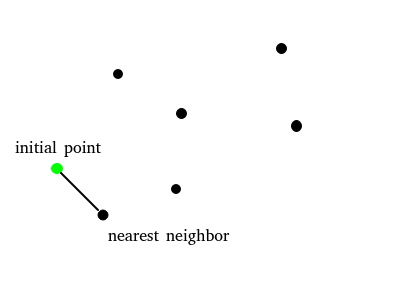
\includegraphics[width=\linewidth]{media/neighbor1.png}
     \caption{Initial step}
  \end{subfigure}
  \begin{subfigure}[b]{0.4\linewidth}
    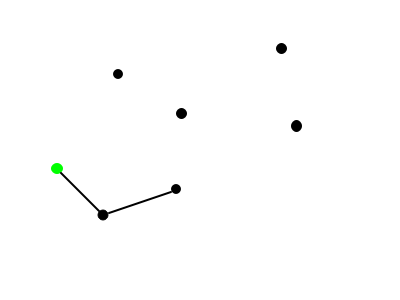
\includegraphics[width=\linewidth]{media/neighbor2.png}
    \caption{Second step}
  \end{subfigure}
  \begin{subfigure}[b]{0.4\linewidth}
    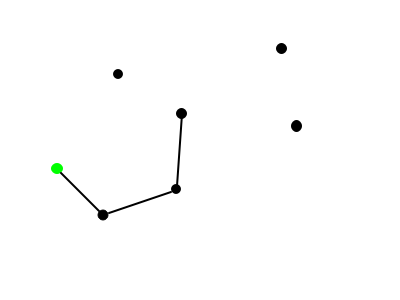
\includegraphics[width=\linewidth]{media/neighbor3.png}
    \caption{Third step}
  \end{subfigure}
  \begin{subfigure}[b]{0.4\linewidth}
    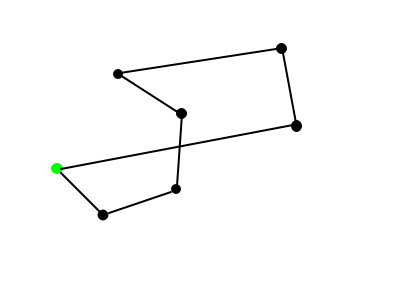
\includegraphics[width=\linewidth]{media/neighbor4.png}
    \caption{Final result}
  \end{subfigure}
  \caption{Execution of nearest neighbor algorithm}
\end{figure}

\noindent On our implementation we decided to trade space for time. Since the operation to compute the nearest point is repeated several time, we decide to store for each point the list of all others points sorted by their distances from that one. This require $O(n^2)$ additional space. Considering the time, instead, to sort the points we implemented a simple \textit{insertion sort}, that is $O(n^2)$, so in total we need an initial $O(n^3)$ (This part could be further improved with a better sort algorithm like \textit{merge sort} that is $O(n \cdot log(n))$, but since the initial time to order the nodes on our experiments was negligible, we decided to use insertion sort that was easier to implement). So, by paying this initial cost we were able to speed up each iteration of nearest neighborhood, in fact each time we needed to find the nearest point we just had to pick the first available one from the ordered list. Of course in the worst case this is $O(n)$, because it can happen that the firsts elements of the ordered list have already been visited, so I have to run across most of the list until I find an available point. However, what we saw in practice is that, except when there are left few nodes to visit, the first available element is always on the firsts position of the ordered list so the operation to find the nearest neighbor became $\Theta(1)$ in most of the cases (for example, we tried on multiple instances between 100 and 500 points and the average number of access to the ordered list to find the nearest point was between 3 and 6). \\

\noindent The major problem of this technique is that visiting always the next closest point leads to the creation of lots of intersection between edges, that of course are inefficient. A possible solution to improve this initial result will be shown on the next section dedicated to the refining algorithms. \\
Another problem is that this algorithm is deterministic, so this mean that if it is run twice starting from the same initial point, it produce the same solution. The consequence of this is that the number of different circuit that it can explore is limited to the total number of nodes.

\subsection{GRASP}
GRASP is a variation of nearest neighborhood that introduce a random component. On each iteration, rather than picking the nearest point to the last visited, select the three closest points and choose one of them at random as next visited vertex. \\
Our implementation was almost the same of nearest neighborhood, with the construction for each point of the initial list of all other points sorted by their distance from that point, with the only difference that first three available points are picked from the list, rather than only one. \\
The introduction of the random component means that the probability to repeat the same sequence starting from the same point is very minimal, so GRASP can explore lots of different circuit resolving the problem of determinism of nearest neighborhood. 

\begin{figure}[h!]
  \centering
  \begin{subfigure}[b]{0.4\linewidth}
    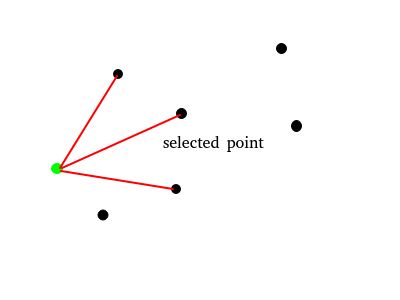
\includegraphics[width=\linewidth]{media/GRASP1.png}
     \caption{Initial step}
  \end{subfigure}
  \begin{subfigure}[b]{0.4\linewidth}
    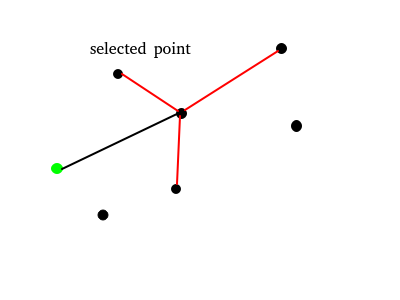
\includegraphics[width=\linewidth]{media/GRASP2.png}
    \caption{Second step}
  \end{subfigure}
  \begin{subfigure}[b]{0.4\linewidth}
    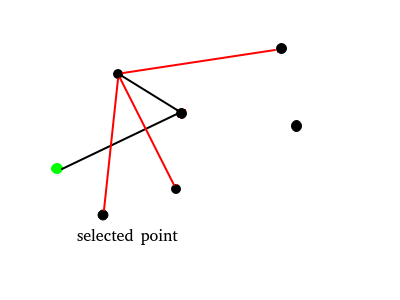
\includegraphics[width=\linewidth]{media/GRASP3.png}
    \caption{Third step}
  \end{subfigure}
  \caption{Execution of 3 steps of GRASP. Each time the 3 closest points are considered and one is picked at random.}
\end{figure}

\subsection{Insertion heuristic}
This algorithm starts from a simple circuit made with only two points. At each iteration, for each of the remaining vertices to insert, compute the minimal extra mileage. The extra mileage is the cost to insert a point on the circuit. So, for example, if we want to insert the vertex z between vertex x and vertex y, the extra mileage is: $c_{xz} + c_{zy} - c_{xy}$, where $c_{ij}$ is the cost of the edge (i, j). The fact that for each point we search the minimal extra mileage means that we are looking to the best position where insert that point. Insert vertex that has the best extra mileage into the partial circuit and repeat the procedure until all the points are inserted. The algorithm than can be executed several time, starting every time from different initial points to explore new solutions and updating the incumbent if necessary. \\
The cost to compute the best extra mileage is $O(n^2)$, so this mean that the entire algorithm is $O(n^3)$.\\
It is also possible to add the GRASP rule, so rather then selecting the point with the best extra mileage, find the three smallest extra mileages and choose at random between them, in this way the algorithm doesn't converge to the same solution starting from the same initial circuit. \\

\begin{figure}[h!]
  \centering
  \begin{subfigure}[b]{0.4\linewidth}
    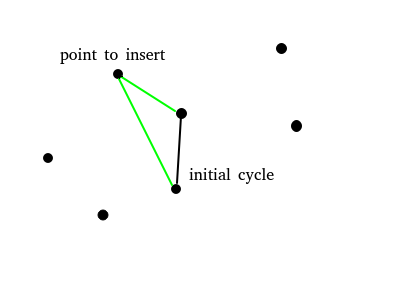
\includegraphics[width=\linewidth]{media/insertion1.png}
     \caption{Initial step}
  \end{subfigure}
  \begin{subfigure}[b]{0.4\linewidth}
    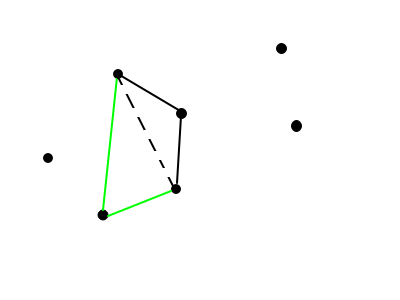
\includegraphics[width=\linewidth]{media/insertion2.png}
    \caption{Second step}
  \end{subfigure}
  \begin{subfigure}[b]{0.4\linewidth}
    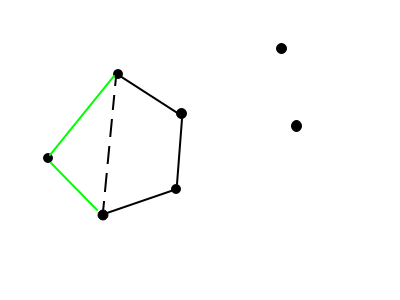
\includegraphics[width=\linewidth]{media/insertion3.png}
    \caption{Third step}
  \end{subfigure}
  \begin{subfigure}[b]{0.4\linewidth}
    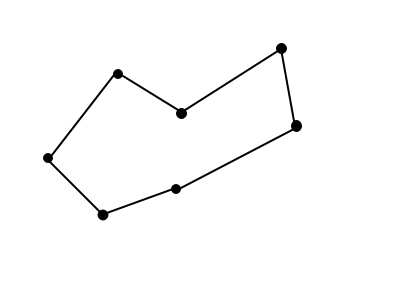
\includegraphics[width=\linewidth]{media/insertion4.png}
    \caption{Final result}
  \end{subfigure}
  \caption{Execution of insertion heuristic algorithm}
\end{figure}

\noindent On our implementation to select the initial circuit we decided to pick at random one point and then to select the furthest point from that one. (Of course this is not the only solution: other possibility are, for example, to pick a vertex and its closest one, or to choose two points completely at random.) I addition, at the beginning of the algorithm, we built a matrix where the element i j contains the distance between vertices i and j (So in total we payed an additional $O(n^2)$ in space). We made this choice because on this algorithm distances between points are computed several times and in addition the same distance can be calculated more than once.\\


\subsection{Insertion with convex hull}
This is a variation of the insertion algorithm. It works in the same way but the initialization is different: rather than starting from an initial cycle made of two random points, compute the convex hull \footnote{In geometry, the convex hull or convex envelope or convex closure of a shape is the smallest convex set that contains it. %TODO AGGIUNGERE CITAZIONE WIKIPEDIA 
} of the instance. Then iterate and insert all the remaining points, that are all inside the convex hull, in the same way of Insertion heuristic.

\section{Refining algorithms}
Refining algorithm are so called because they start from an admissible solution that could by provided by any other algorithm and they try to improve it with a series of iteration.

\subsection{TWO-OPT}
The first algorithm we present is TWO-OPT (or 2-OPT). To explain this technique, let's consider two edges, the first delimited by vertices a and b and with cost $c_{ab}$, the second delimited by c and d and with cost $c_{ab}$ (Both edges belong to an admissible solution provided by any algorithm). Now let's swap the two edges: as result we obtain the edges a, c and b, d with cost respectively $c_{ac}$ and $c_{bd}$. Now lets compute: 
\begin{equation*}
\Delta = c_{ab} + c_{ab} - (c_{ac} + c_{bd})
\end{equation*}
that is the cost of the initial edges minus the cost of the swapped edges. If $\Delta > 0$, it means that the new edges are better than the older and the swap is worth because it reduce (improve) the objective function. Of course the new solution produced is still admissible.\\

\begin{figure}[h!]
\centering
	\begin{tabular}{@{}cccc@{}}
		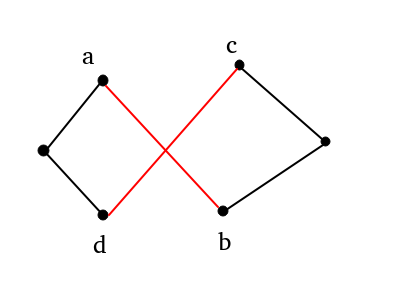
\includegraphics[scale=0.6]{media/2-opt1.png} &
		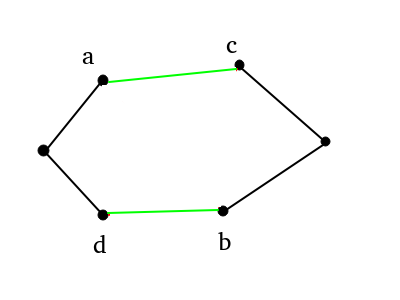
\includegraphics[scale=0.6]{media/2-opt2.png} \\
	\end{tabular}
	\caption{The 2-OPT move, edges in red are removed and replaced by green edges.}
\end{figure}

\noindent 2-OPT works in this way: start from an admissible solution, consider all the possible couple of edges (that are in total $O(n^2)$) and for each of them compute the $\Delta$ (That can be calculated in $\Theta(1)$). Then pick the largest $\Delta$ and swap the relatives edges. After this operation, one of the two parts of the cycle that has been divided by the swap, need to be retraced in order to invert the visit sequence of the vertices and reconnect it to the new edge (This is $O(n)$, but since it is done after a $O(n^2)$ doesn't change the overall cost of the swap). Repeat the procedure until all the $\Delta$ are negative, or a fixed time limit is reached.\\

\noindent This algorithm is very good to remove edge intersections, like the ones produced  by nearest neighborhood (or GRASP). Here in the table below some examples.\\

\begin{table}[h!]
	\begin{center}
		\begin{tabular}{l|c|c|c}
			\textbf{Instance} & \textbf{GRASP} & \textbf{2-OPT} & \textbf{Improve}	\\
			& (5 sec) & (5 sec) & \\
			\hline
			att48 & 41806 & 35522 & 15\% \\
			eil101 & 879 & 691 & 21\% \\
			ch130 & 9801 & 6347 & 35\% \\
			ch150 & 10477 & 7278 & 30\% \\
			a280 & 4546 & 2886 & 36\% \\
			lin318 & 76940 & 46235 & 39\% \\ 
			att532 & 155010 & 97487 & 37\% \\	
			pr1002 & 492311 & 285078 & 42\% \\
		\end{tabular}
		\caption{Values of the objective functions after running on each instance GRASP algorithm for 5 seconds and then 2-OPT for other 5 seconds.}
	\end{center}
\end{table}

\noindent These results were obtained after running GRASP for five seconds and then refining the solution with 2-OPT for other five seconds. Of course this dataset is very small but it gives the idea of the power of this technique, we have, in fact, a significant improve of the objective function in all the cases. To notice that the improve increase with large problem. \\
It is possible to visualize the action of 2-OPT by plotting the solution before and after the refining:

\begin{figure}[h!]
\centering
	\begin{tabular}{@{}cccc@{}}
		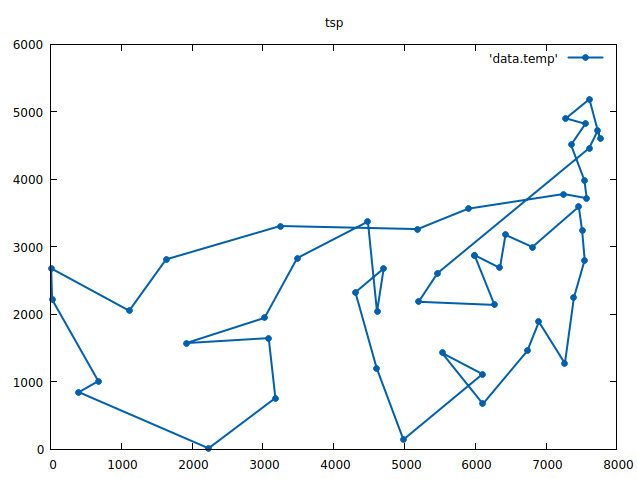
\includegraphics[scale=0.40]{media/before2opt.png} \\
		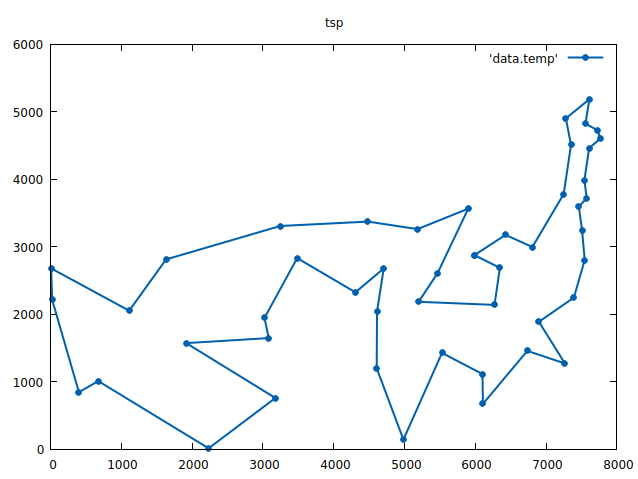
\includegraphics[scale=0.40]{media/after2opt.png} \\
	\end{tabular}
	\caption{Solution of 5 sec of GRASP before (top image) and after (bottom image) a refining of 5 sec}
\end{figure}


\subsection{THREE-OPT}
3-OPT is a variation of 2-OPT that consider 3 edges for the swap rather than only two. This time there are multiple way to combine the 3 selected edges, in particular for a triad there are 7 possible moves. Moreover, I have to consider all the possible triad to find the best one and this is $O(n^3)$. So in general 3-OPT is more complicated to implement and due to the fact that is cubic doesn't work well with big problems, for example with instances with more than 10000 points.

\section{Meta-heuristics}
\subsection{Variable neighborhood search}
After performing a refinement technique, like 2-OPT, if the time limit is not reached, the algorithm stop on a local minima of the objective function. Now, a possibility, is to restart from the beginning providing another initial solution and refining it, until a new local minima is reached, with the hope that it will better than the previous one (GRASP + 2-OPT works in this way). Of course this is not an efficient solution because each time I restart all the work done on the previous execution is unused. \\
Variable neighborhood search (VNS) provide a simple yet powerful way to escape the local minima. Let's assume that we have completed the refinement using 2-OPT. At this point we can perform a random move with a bigger research radius, a 3-OPT or a 5-OPT for example. Since this move is completely random, it will make the solution worse but it will also provide the "kick" that we need to escape the local minima. Now we can restart with 2-OPT until a new minima is found (that could also be the optimum).\\
In synthesis, VNS, works with two phases that alternate continuously: an intensification  phase (2-OPT) where the algorithm move toward a minima and a diversification phase where VNS perform a 3-OPT or greater random move to exit from the minima.
\subsection{Tabu search}
Tenure = dim tabù list
\subsection{Simulated Annealing}
\subsection{Multi-start}
\subsection{Genetic Algorithm}
